%--------------------------------------------------------------------
%  Capítulo 3 · Aportaciones del Proyecto Tutor Virtual
%--------------------------------------------------------------------
\chapter{Aportaciones del Proyecto}
\label{chap:aportaciones}
\justifying

Este capítulo detalla las contribuciones del proyecto, tanto desde una perspectiva técnica como pedagógica. 

Se inicia con una visión general de la arquitectura del sistema, seguida de una descripción de las aportaciones específicas en el diseño del modelo de datos, el pipeline de inteligencia artificial, el desarrollo del backend y del frontend. 

Por último, se enumeran las contribuciones en el ámbito pedagógico, las limitaciones identificadas en la implementación actual y un resumen de las líneas de trabajo futuro.

%--------------------------------------------------------------------
\section{Visión General de la Arquitectura y Componentes}
\label{sec:vision_general_aportaciones}

\noindent
El sistema ha sido diseñado como una aplicación multicapa que integra los componentes de inteligencia artificial local, el servidor backend y la interfaz de usuario frontend. Esta arquitectura busca cerrar el ciclo interactivo: \emph{estudiante \(\rightarrow\) ejercicio \(\rightarrow\) feedback \(\rightarrow\) métrica de progreso}. La Figura~\ref{fig:overview-tutorvirtual} ofrece una representación de alto nivel de esta estructura.

\begin{figure}[H]
  \centering
  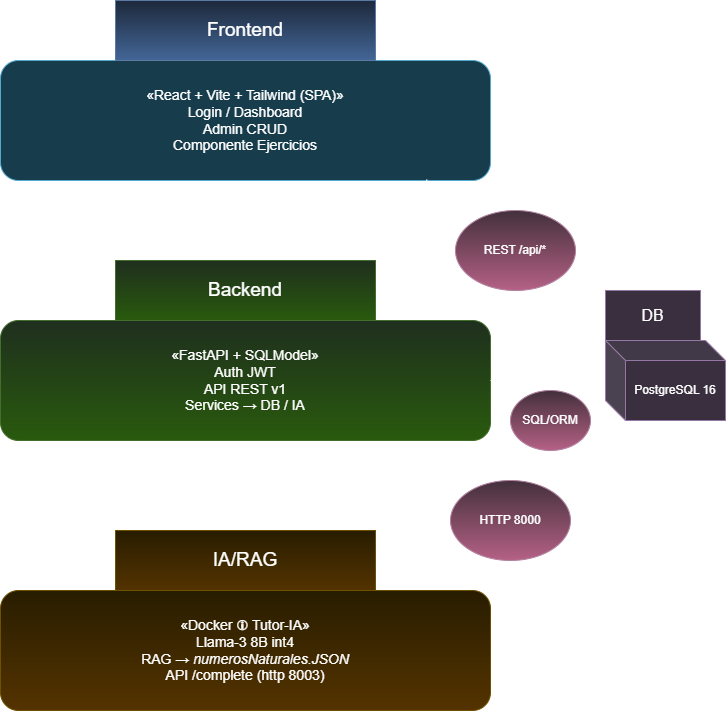
\includegraphics[width=.9\linewidth]{Ilustraciones/overview_tutorvirtual.png}
  \caption[Arquitectura en capas de Tutor Virtual]{Vista de la arquitectura en capas de \textbf{Tutor Virtual}, resaltando los flujos principales de datos y control entre el frontend, el backend y el motor de IA local.}
  \label{fig:overview-tutorvirtual}
\end{figure}

Las principales aportaciones se pueden agrupar en tres bloques:
\begin{itemize}
    \item \textbf{Aportación 1 (Frontend React):} Desarrollo de una interfaz de usuario intuitiva y reactiva construida con \texttt{Vite + React + TailwindCSS}. Con componentes reutilizables clave como \texttt{MultiCheckList} para selección múltiple y un panel de progreso para el estudiante.
    \item \textbf{Aportación 2 (Backend RESTful):} Implementación de un servidor API REST utilizando \texttt{FastAPI + PostgreSQL}. Este backend gestiona la lógica de negocio, las operaciones CRUD (Crear, Leer, Actualizar, Borrar) sobre los datos, la autenticación de usuarios mediante JWT (JSON Web Tokens) y el registro de interacciones e intentos.
    \item \textbf{Aportación 3 (Motor de IA Local):} Uso de un motor de inteligencia artificial, desplegado en un contenedor Docker. Este motor utiliza el modelo \texttt{llama-3-8B-int4.gguf} junto con técnicas de Recuperación Aumentada por Generación (RAG) para generar ejercicios y proporcionar explicaciones personalizadas, todo ello ejecutándose localmente.
\end{itemize}

%--------------------------------------------------------------------
\section{Contribuciones Técnicas Detalladas}
\label{sec:contribuciones_tecnicas}

A continuación, se describen con mayor detalle las aportaciones técnicas específicas del proyecto.

%--------------------------------------------------------------------
\subsection{Modelo de Datos Optimizado y Flexible}
\label{ssec:datamodel_aportaciones}

Se ha diseñado e implementado un modelo de datos relacional (ver Figura~\ref{fig:er-diagram}) que, manteniendo la simplicidad, ofrece la flexibilidad necesaria para la gestión de la información académica. Destaca el soporte para relaciones \(\texttt{N:M}\) (muchos a muchos) entre cursos y asignaturas, permitiendo que una asignatura pueda pertenecer a múltiples cursos y viceversa. Asimismo, se establece una relación \(\texttt{1:N}\) (uno a muchos) entre asignaturas y temas, estructurando jerárquicamente el contenido educativo. Este diseño facilita la escalabilidad y la organización del material pedagógico.

\begin{figure}[H]
  \centering
  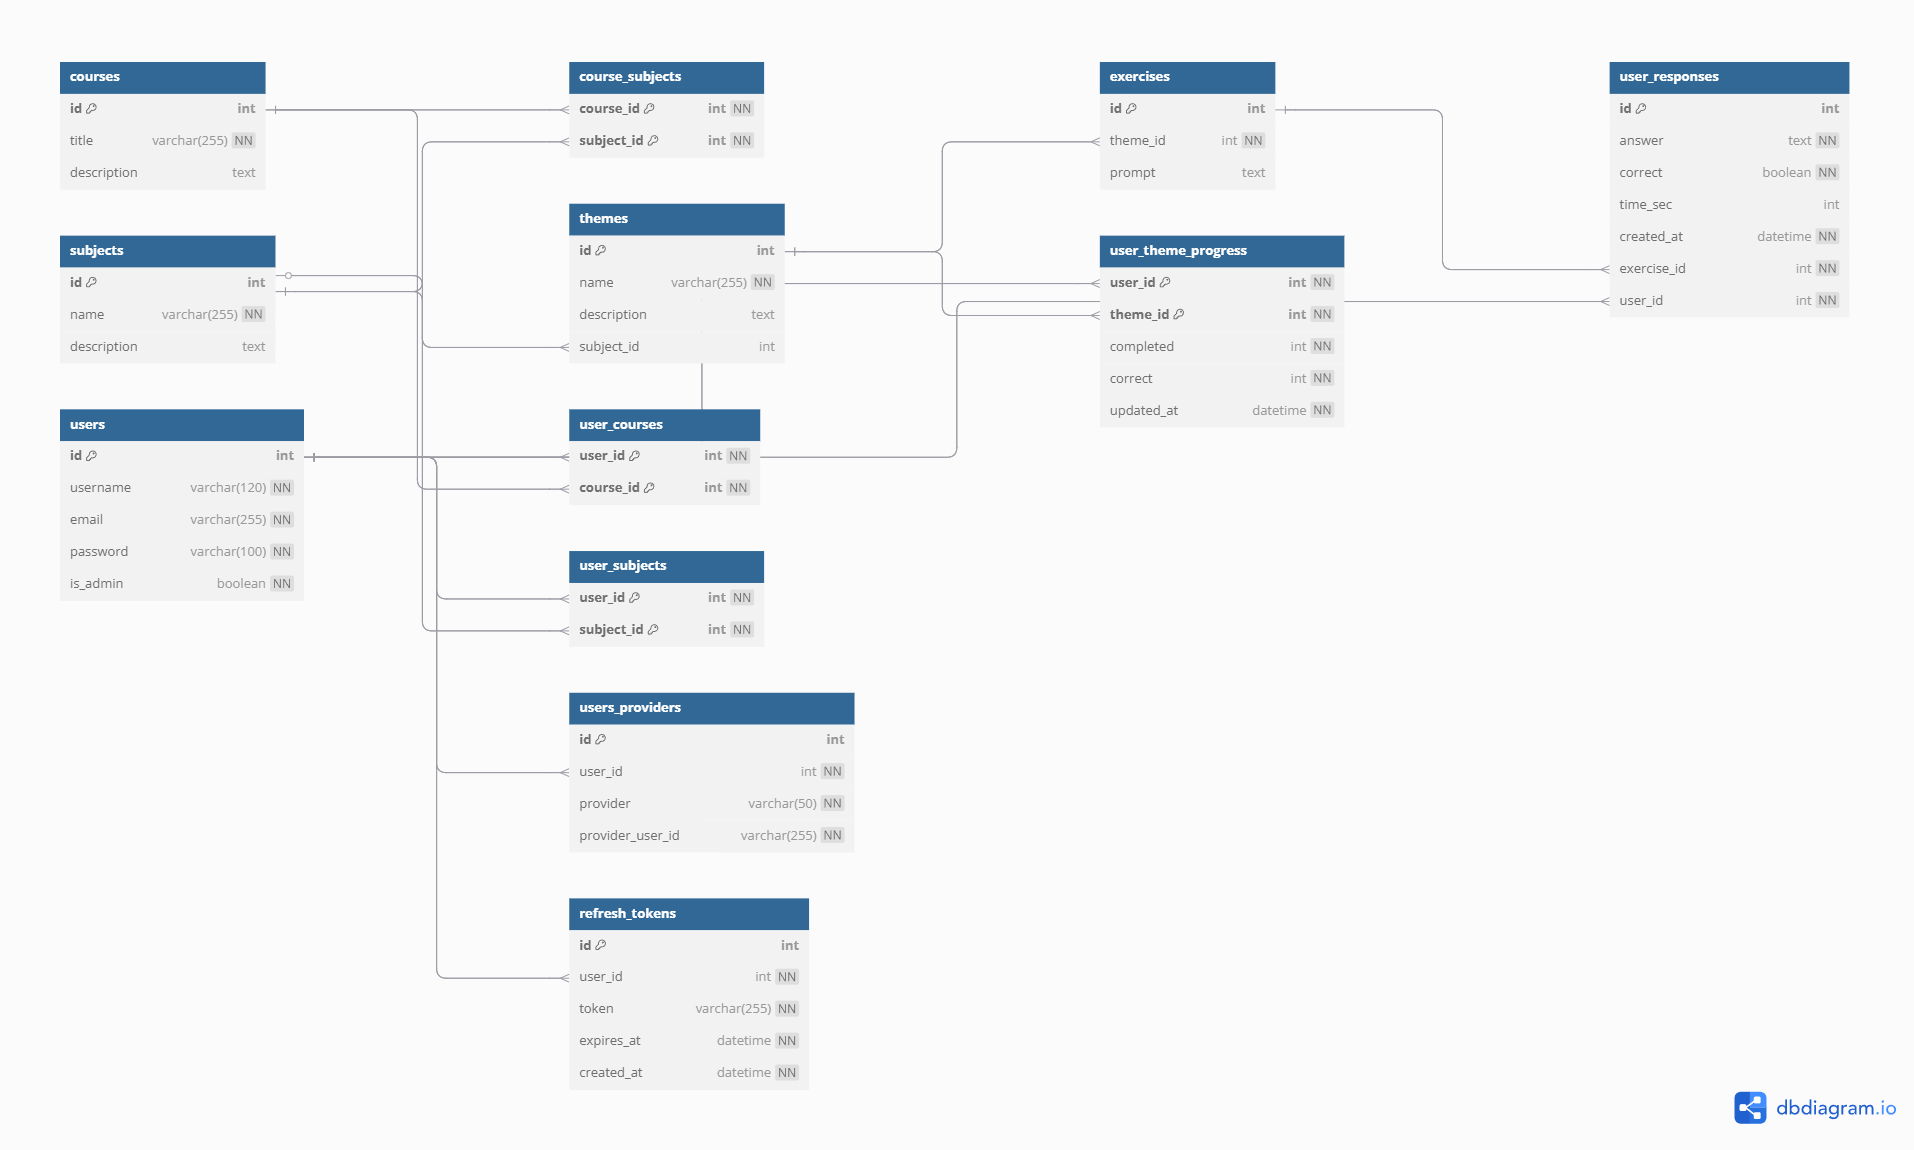
\includegraphics[width=.9\linewidth]{Ilustraciones/er_diagram.png}
  \caption{Diagrama Entidad-Relación (E-R) final implementado en Tutor Virtual, mostrando las tablas principales y sus interrelaciones.}
  \label{fig:er-diagram}
\end{figure}

%--------------------------------------------------------------------
\subsection{Pipeline de Inteligencia Artificial con RAG y Ejecución Local}
\label{ssec:pipeline_ia_aportaciones}

Una de las aportaciones centrales es el desarrollo de un pipeline de IA completamente local:
\begin{enumerate}[label=\alph*),leftmargin=*]
  \item \textbf{Creación de un \textit{dataset} propio para RAG}: Se ha compilado y estructurado un conjunto de datos específico para el dominio educativo inicial (ejercicios de matemáticas sobre números naturales, almacenados en archivos como \texttt{numerosNaturales.txt}). Este \textit{dataset}, con más de \SI{300}{} ejemplos, sirve como base para la recuperación de contexto en el sistema RAG, mejorando la precisión de las respuestas generadas.
  \item \textbf{Desarrollo de un Contenedor IA autocontenido}: Se ha construido una imagen Docker que empaqueta el modelo LLM, el motor de inferencia \texttt{llama.cpp}, y el entorno Python 3.11 con las bibliotecas necesarias para el RAG y la API interna del motor. Esto asegura la portabilidad y reproducibilidad del componente de IA.
  \item \textbf{Optimización del tiempo de inferencia (\emph{Warm-up} y uso continuo)}: Aunque la primera inferencia tras el inicio del contenedor puede tardar entre 7 y 10 segundos (fase de \emph{warm-up} y carga del modelo en memoria), las inferencias siguientes se han alcanzan tiempos de respuesta aceptables.
\end{enumerate}

\subsubsection*{Ejemplo de Plantilla de Prompt para Generación de Ejercicios}
\label{sssec:ejemplo_prompt}
Para la comunicación con el LLM, se utilizan plantillas de \emph{prompt}. El Listado~\ref{lst:prompt_aportaciones} muestra un ejemplo simplificado en formato JSON utilizado para solicitar la generación de un ejercicio.

\begin{lstlisting}[language=java,caption={Ejemplo de plantilla de prompt (formato JSON simplificado) para la generación de ejercicios.},label={lst:prompt_aportaciones},basicstyle=\fontsize{8}{9.5}\ttfamily]
{
  "model": "profesor_generador_ejercicios",
  "response_format": { "type": "json_object" },
  "messages": [
    {
      "role": "user",
      "content": "Genera un ejercicio sobre el tema \"{{theme.title}}\" con un nivel de dificultad {{difficulty}}. El formato de la respuesta esperada debe ser {{exercise_response_type}}. "
    }
  ]
}
\end{lstlisting}

%--------------------------------------------------------------------
\subsection{Backend Robusto y Escalable con FastAPI}
\label{ssec:backend_aportaciones}

El backend, desarrollado con FastAPI, proporciona una API RESTful completa para la gestión de la plataforma. Algunas características son:
\begin{itemize}
    \item \textbf{Gestión modular de entidades:} Implementación de rutas CRUD para todas las entidades principales del sistema (usuarios, cursos, asignaturas, temas, ejercicios, respuestas).
    \item \textbf{Autenticación y autorización seguras:} Uso de JWT para la autenticación de usuarios y protección de rutas sensibles, asegurando que solo usuarios autorizados puedan acceder o modificar ciertos recursos.
    \item \textbf{Validación de datos con Pydantic:} Aprovechamiento de los modelos de Pydantic para la validación automática de los datos de entrada y salida de la API, mejorando la robustez y fiabilidad del sistema.
    \item \textbf{Registro (logging) exhaustivo:} Implementación de un sistema de logging para registrar los intentos de los estudiantes, interacciones con la IA y eventos importantes del sistema, útil para depuración, análisis y futuras auditorías.
\end{itemize}
La Tabla~\ref{tab:endpoints_aportaciones} muestra un ejemplo de los endpoints implementados. Un detalle más exhaustivo de la API se encuentra en el Capítulo~\ref{chap:desarrollo} (Desarrollo del Proyecto).

\begin{table}[H]
  \centering
  \begin{tabularx}{\linewidth}{@{} l l X @{}}
    \toprule
    \textbf{Verbo HTTP} & \textbf{Ruta API} & \textbf{Descripción Funcional} \\ 
    \midrule
    GET    & \texttt{/api/course/courses}                             & Obtiene la lista de todos los cursos disponibles. \\
    POST   & \texttt{/api/subjects/create}                            & Crea una nueva asignatura en el sistema. \\
    POST   & \texttt{/api/subjects/courses/\{course\_id\}/subjects/add}      & Vincula una asignatura existente a un curso específico. \\
    GET    & \texttt{/api/subjects/\{subject\_id\}/themes}     & Lista los temas asociados a una asignatura. \\
    POST   & \texttt{/api/ai/request}& Solicita la generación de un ejercicio para un tema y dificultad. \\
    \bottomrule
  \end{tabularx}
  \caption{Ejemplo de algunos de los endpoints de la API REST implementados en el backend.}
  \label{tab:endpoints_aportaciones}
\end{table}

%--------------------------------------------------------------------
\subsection{Frontend Interactivo y Centrado en el Usuario}
\label{ssec:frontend_aportaciones}

El frontend se ha desarrollado con un enfoque en la usabilidad y la experiencia del usuario:
\begin{itemize}[leftmargin=*]
  \item \textbf{Componente \texttt{MultiCheckList}:} Se diseñó y desarrolló un componente React específico, \texttt{MultiCheckList}, que presenta una lista de ítems (ej. asignaturas, temas) con casillas de verificación internas. Este componente simplifica la interfaz para selecciones múltiples complejas y es reutilizable en diferentes partes de la aplicación.
  \item \textbf{Optimización del \texttt{AdminDashboard} con invalidación de caché selectiva:} Para el panel de administración, se implementó una estrategia de invalidación de caché más eficiente utilizando \texttt{queryClient.refetchQueries} de React Query. Esto permite actualizar los datos de forma selectiva e inmediata tras una mutación, en lugar de depender únicamente de un \emph{polling} periódico (ej. cada 5 segundos).
  \item \textbf{Sistema de notificaciones (\emph{Toasts}) personalizable:} Se creó un sistema de notificaciones (mensajes emergentes o \emph{toasts}) utilizando el contexto de React y CSS utilitario (TailwindCSS), sin necesidad de introducir dependencias externas. Estas notificaciones se utilizan para informar al usuario sobre el resultado de las operaciones (éxito, error, advertencia).
\end{itemize}

%--------------------------------------------------------------------
\section{Contribuciones Pedagógicas Clave}
\label{sec:contribuciones_pedagogicas}

Más allá de los aspectos técnicos, Tutor Virtual introduce las siguientes aportaciones de valor pedagógico:
\begin{enumerate}[leftmargin=*]
  \item \textbf{Banco de ejercicios con niveles de dificultad:} El sistema permite la creación y gestión de ejercicios clasificados explícitamente por niveles de dificultad, proporcionando a los estudiantes una estructura clara para su aprendizaje.
  \item \textbf{Fomento de la autonomía del estudiante mediante selector explícito de dificultad:} Como se discutió en el Capítulo~\ref{chap:estado_arte_enfoque}, la capacidad de que el estudiante seleccione conscientemente la dificultad de los ejercicios busca potenciar su sentido de autonomía y autoeficacia.
  \item \textbf{Retroalimentación inmediata y generada por IA:} El sistema provee \emph{feedback} instantáneo sobre las respuestas de los estudiantes. Esta retroalimentación es generada por el LLM local, permitiendo comentarios más elaborados y contextualizados que los sistemas tradicionales basados en respuestas predefinidas.
\end{enumerate}


%--------------------------------------------------------------------
\section{Limitaciones Actuales Identificadas}
\label{sec:limitaciones_actuales_aportaciones}

A pesar de los avances logrados, el prototipo actual de Tutor Virtual presenta ciertas limitaciones:
\begin{description}[leftmargin=*, style=unboxed,font=\normalfont]
  \item[Limitaciones Técnicas:]\\
    \begin{itemize}
        \item El tiempo de \emph{warm-up} inicial del motor de IA puede ser perceptible para el primer usuario o tras un reinicio.
        \item El panel de administración podría beneficiarse de actualizaciones en tiempo real mediante WebSockets en lugar de depender de \emph{polling} o invalidación manual para ciertos datos.
        \item La gestión de errores y la robustez del pipeline de IA pueden requerir mayor refinamiento para casos borde.
    \end{itemize}
  \item[Limitaciones No Técnicas (Ámbito y Cumplimiento):]\\
    \begin{itemize}
        \item No se ha implementado un módulo específico para la gestión del consentimiento explícito del RGPD, más allá de la privacidad inherente al diseño local.
        \item No se ha realizado una auditoría ética formal del sistema ni de los contenidos generados por la IA, lo cual sería un paso importante para un despliegue a mayor escala.
        \item El contenido pedagógico actual está limitado al dominio inicial de prueba (matemáticas básicas).
    \end{itemize}
\end{description}

%--------------------------------------------------------------------
\section{Resumen de Líneas de Trabajo Futuro}
\label{sec:trabajo_futuro_resumen_aportaciones}

Las limitaciones actuales y el potencial del sistema abren diversas vías para trabajos futuros. Estas se detallarán extensamente en el Capítulo~\ref{chap:conclusiones} (Conclusiones y Trabajo Futuro), pero se resumen a continuación:
\begin{enumerate}[label=\arabic*),leftmargin=*]
  \item Implementación de evaluación de respuestas abiertas con verificación semántica más avanzada, yendo más allá de la simple comparación de respuestas exactas.
  \item Externalización y versionado de las plantillas de \emph{prompt} (por ej. utilizando ficheros YAML o JSON externos) para facilitar su gestión y experimentación.
  \item Desarrollo de un módulo completo de cumplimiento RGPD, incluyendo gestión de consentimiento informado, derecho al olvido y portabilidad de datos.
  \item Exploración de la migración de ciertas funcionalidades (como la actualización de métricas en el panel de progreso) a WebSockets para una interactividad en tiempo real más eficiente.
  \item Ampliación del banco de contenidos a otras asignaturas y niveles educativos.
  \item Investigación sobre la interpretabilidad de las respuestas del LLM (\emph{Explainable AI - XAI}) adaptada al contexto educativo.
\end{enumerate}

